\begin{frame}[fragile]
\frametitle{Пример}
\pause
\begin{lstlisting}
RandomGenerator rng;
int hits = 0;
for (int i = 0; i < nSamples; i++) {
   float x = rng.getUniform();
   float y = rng.getUniform();
   int res = x*x + y*y < 1.0f ? 1 : 0;
   hits += res;
}
float final = hits * 4.0f / nSamples;
\end{lstlisting}
\end{frame}

\begin{frame}
  \frametitle{$\pi$ - Монте Карло}
  \begin{figure}[t]
    \animategraphics[height=7.5cm,loop,autoplay]{2}{animated/pi_frame-}{0}{9}
%    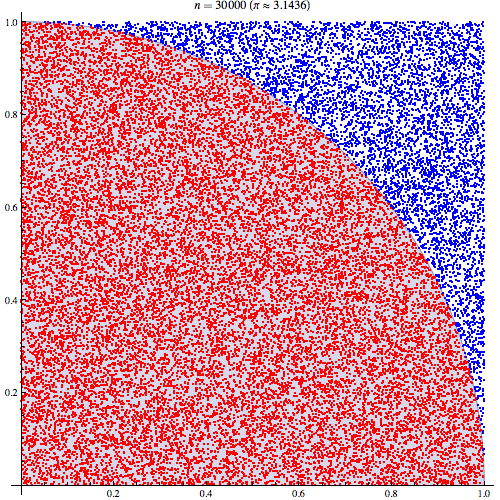
\includegraphics[height=7.5cm]{pi_frame-9.png}
  \end{figure}
\end{frame}

\begin{frame}
  \frametitle{$\pi$ - Монте Карло}
  \begin{equation*}
   h(x,y) = \begin{cases}
        1,& \text{ако } x^2 + y^2 < 1 \\
        0,& \text{иначе}\\
        \end{cases}
  \end{equation*}
  \pause

  \begin{equation*}
    \Omega = x \in [0 .. 1] \times y \in [0 .. 1]
  \end{equation*}
  \pause

  \begin{equation*}
   \int_{\Omega} h(x,y) dx dy = \frac{\pi}{4} \Rightarrow 
  \end{equation*}
  \pause
  \begin{equation*}
   \pi = 4 \int_{\Omega} h(x,y) dx dy
  \end{equation*}
\end{frame}
